\documentclass[11pt, english, fleqn, DIV=15, headinclude, BCOR=1.5cm]{scrartcl}

\usepackage[
    bibatend,
    color,
]{../header}

\usepackage{tikz}
\usepackage{pdflscape}

\usepackage[tikz]{mdframed}
\newmdtheoremenv[%
    backgroundcolor=black!5,
    innertopmargin=\topskip,
    splittopskip=\topskip,
]{theorem}{Theorem}[section]

\hypersetup{
    pdftitle=
}

\newcounter{totalpoints}
\newcommand\punkte[1]{#1\addtocounter{totalpoints}{#1}}

\newcounter{problemset}
\setcounter{problemset}{8}

\subject{physics606 -- Advanced Quantum Theory}
\ihead{physics606 -- Problem Set \arabic{problemset}}

\title{Problem Set \arabic{problemset}}

\publishers{Group 2 -- Dilege Gülmez}
\ofoot{Group 2 -- Dilege Gülmez}

\newmdenv[%
    backgroundcolor=black!0,
    frametitlebackgroundcolor=black!0,
    roundcorner=5pt,
    skipabove=\topskip,
    innertopmargin=\topskip,
    splittopskip=\topskip,
    frametitle={Problem statement},
    frametitlerule=true,
    nobreak=true,
]{problem}

\newmdenv[%
    backgroundcolor=white,
    frametitlebackgroundcolor=black!0,
    roundcorner=5pt,
    skipabove=\topskip,
    innertopmargin=\topskip,
    innerbottommargin=8cm,
    splittopskip=\topskip,
    frametitle={Side question},
    frametitlerule=true,
]{question}

\newcommand\an{^\text{angular}}
\newcommand\ra{^\text{radial}}


\author{
    Martin Ueding \\ \small{\href{mailto:mu@martin-ueding.de}{mu@martin-ueding.de}}
    \and
    Lino Lemmer \\ \small{\href{mailto:l2@uni-bonn.de}{l2@uni-bonn.de}}
}
\ifoot{Martin Ueding, Lino Lemmer}

\ohead{\rightmark}

\begin{document}

\maketitle

\vspace{3ex}

\begin{center}
    \begin{tabular}{rrr}
        problem number & achieved points & possible points \\
        \midrule
        1 & & \punkte{14} \\
        2 & & \punkte{15} \\
        \midrule
        total & & \arabic{totalpoints}
    \end{tabular}
\end{center}

\section{Wave packet}

We again write vectors in bold type, like $\vec k$, as opposed to scalars in
regular italic font, like $k$. We also adopt the notation that $k = |\vec k|$.

\subsection{Phase velocity}

The phase of a single plane wave has to be constant, so
\[
    \vec k \vec x - \omega(k) t = c_1.
\]
The total time derivative has to be zero, then. $\vec k$ is constant for a
monochrome wave. This means
\begin{align*}
    \vec k \dot{\vec x} &= \omega(k). \\
    \iff k \frac{\vec k}{k} \dot{\vec x} &= \omega(k) \\
    \iff \frac{\vec k}{k} \dot{\vec x} &= \frac{\omega(k)}k \\
    \intertext{%
        The part of the velocity that is in the direction of $\vec k$ is given
        by the right hand side. Since the propagation is taken to be this $\vec
        k$ direction, we can just write down the projection onto $\vec k$.
    }
    \iff \vec v_\text{ph} &= \frac{\vec k}{k} \frac{\omega(k)}k
\end{align*}

\subsection{Group velocity}

We start by inserting $\vec k = \vec k_0 + \vec \delta$ into equation~(1) from
the problem set.
\begin{align*}
    \psi(\vec x, t)
    &= \int \frac{\dif^3 \delta}{[2\piup]^3} a(\vec k_0 + \vec \delta)
    \exp\del{
        \iup \sbr{
            [\vec k_0 + \vec \delta] \vec x - \omega\del{|\vec k_0 + \vec
            \delta|} t
        }
    }
    \intertext{%
        We expand the angular frequency around $\vec \delta = \vec 0$:
        \[
            \omega\del{|\vec k_0 + \vec \delta|}
            = \omega(k_0) + \od\omega k \vec \delta \frac{\vec k_0}{k_0} + \mathcal O(\delta^2)
        \]
        We insert this into the integral up to first order.
    }
    &\approx \int \frac{\dif^3 \delta}{[2\piup]^3} a(\vec k_0 + \vec \delta)
    \exp\del{
        \iup \sbr{
            [\vec k_0 + \vec \delta] \vec x - \sbr{
                \omega(k_0) + \od\omega k \vec \delta \frac{\vec k_0}{k_0}
            }
            t
        }
    }
    \intertext{%
        The parts that depend on $\vec \delta$ are taken out front.
    }
    &=
    \exp\del{
        \iup \sbr{
            \vec k_0 \vec x - \omega(k_0) t
        }
    }
    \int \frac{\dif^3 \delta}{[2\piup]^3} a(\vec k_0 + \vec \delta)
    \exp\del{
        \iup \sbr{ \vec \delta \vec x - \od\omega k \vec \delta \frac{\vec
        k_0}{k_0} t }
    }
    \intertext{%
        Now we can do the same thing as in the first problem where we have
        factored out $\vec k$.
    }
    &=
    \exp\del{
        \iup \vec k_0 \sbr{ \vec x - v_\text{ph} t }
    }
    \int \frac{\dif^3 \delta}{[2\piup]^3} a(\vec k_0 + \vec \delta)
    \exp\del{
        \iup \sbr{ \vec \delta \vec x - \od\omega k \vec \delta \frac{\vec
        k_0}{k_0} t }
    }
    \intertext{%
        The next thing is to factor out the $\vec \delta$.
    }
    &=
    \exp\del{
        \iup \vec k_0 \sbr{ \vec x - v_\text{ph} t }
    }
    \int \frac{\dif^3 \delta}{[2\piup]^3} a(\vec k_0 + \vec \delta)
    \exp\del{
        \iup \vec \delta \sbr{ \vec x - \od\omega k \frac{\vec
        k_0}{k_0} t }
    }
    \intertext{%
        This is the form that we had to show for the given hint when
        equation~(4) from the problem set it inserted.
    }
    &=
    \exp\del{
        \iup \vec k_0 \sbr{ \vec x - v_\text{ph} t }
    }
    \int \frac{\dif^3 \delta}{[2\piup]^3} a(\vec k_0 + \vec \delta)
    \exp\del{
        \iup \vec \delta \sbr{ \vec x - v_\text{gr} t }
    }
\end{align*}

\subsection{Time evolution}

It is easiest to write this as ratio of the given ones. The only difference is
the velocity in the first exponential function.
\begin{align*}
    \frac{\psi(\vec x, t)}{\psi(\vec x - \vec v_\text{gr} t, 0)}
    &\approx
    \frac{
        \exp\del{
            \iup \vec k_0 \sbr{ \vec x - v_\text{ph} t }
        }
        \int \frac{\dif^3 \delta}{[2\piup]^3} a(\vec k_0 + \vec \delta)
        \exp\del{
            \iup \vec \delta \sbr{ \vec x - v_\text{gr} t }
        }
    }
    {
        \exp\del{
            \iup \vec k_0 \sbr{ \vec x - v_\text{gr} t }
        }
        \int \frac{\dif^3 \delta}{[2\piup]^3} a(\vec k_0 + \vec \delta)
        \exp\del{
            \iup \vec \delta \sbr{ \vec x - v_\text{gr} t }
        }
    }
    \intertext{%
        This can be simplified since the integrals are just the exact same.
    }
    &=
    \frac{
        \exp\del{
            \iup \vec k_0 \sbr{ \vec x - v_\text{ph} t }
        }
    }
    {
        \exp\del{
            \iup \vec k_0 \sbr{ \vec x - v_\text{gr} t }
        }
    }
    \intertext{%
        The remainder is easy, just put the two exponentials together
    }
    &=
    \exp\del{
        \iup \vec k_0 \sbr{ \vec v_\text{gr} - v_\text{ph} } t
    }
\end{align*}
This can then we rewritten in the form of equation~(6) from the problem set.

\subsection{Massless and massive particles}

The relation between energy and angular frequency is given by
\[
    E(k) = \hbar \omega(k).
\]

\subsubsection{Massless particle}

We have
\[
    \omega = ck
\]
in this case. Therefore
\[
    v_\text{ph} = v_\text{gr} = c
\]
which is not really surprising for a massless particle which has to propagate
with the speed of light regardless of this energy.

\subsubsection{Massive particle}

Here
\[
    E = \frac{\hbar^2 k^2}{2m}
\]
such that
\[
    \omega = \frac{\hbar k^2}{2m}.
\]
Then
\[
    v_\text{ph} = \frac{\hbar k}{2m}
    \eqnsep
    v_\text{gr} = \frac{\hbar k}{m}.
\]

When this is inserted into the phase factor, one gets the desired result after
a few simplifications which are hardly worth mentioning here.

\subsection{Relativistic particle}

The angular frequency is
\[
    \omega(k) = \frac{1}{\hbar} \sqrt{M^2 c^4 + \hbar^2 k^2 c^2}.
\]
From this, computing the velocities can be derived without new principles:
\[
    v_\text{ph} = \frac{1}{\hbar k} \sqrt{M^2 c^4 + \hbar^2 k^2 c^2}
    \eqnsep
    v_\text{gr} = \frac{\hbar}{\sqrt{M^2 c^4 + \hbar^2 k^2 c^2}} h c^2
\]
Taking the limits is not really difficult since nothing diverges. We obtain
\[
    \lim_{M \to 0} v_\text{ph} = c
    \eqnsep
    \lim_{M \to 0} v_\text{gr} = c
    \eqnsep
    \lim_{k \to 0} v_\text{gr} = 0.
\]

\section{Scattering on a constant potential}

\subsection{Scattering amplitude}

Given is
\[
    f_{\vec k}(\theta) = - \frac{2MV_0}{q \hbar^2} \int_0^\infty \dif r' \, r
    \sin(qr')
\]
and the following potential:
\[
    V(\vec x) =
    \begin{cases}
        V_0 & x < r_0 \\
        0 & \text{else}
    \end{cases}
\]
In this part of the problem, we have to compute $f_{\vec k}$ explicitly.

Well, this does not make too much sense as the problem is posed. The integral
does not converse, since the integrand oscillates badly, see
figure~\ref{fig:divergence}. It is not \emph{Mathematica} integrable either.

\begin{figure}[htbp]
    \centering
    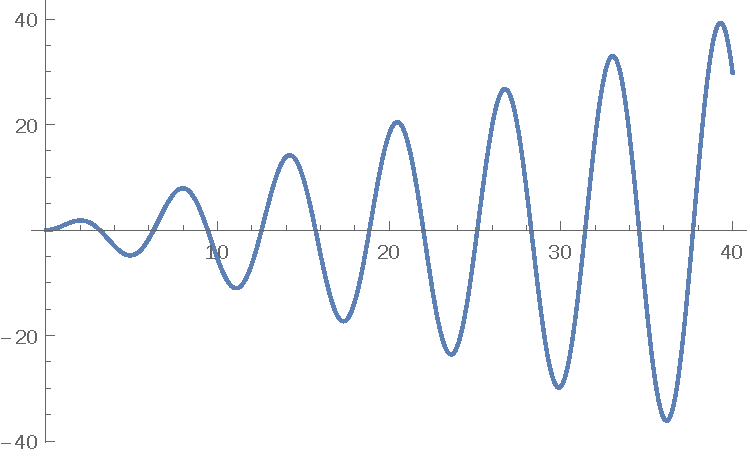
\includegraphics[width=.7\linewidth]{divergence.pdf}
    \caption{%
        Plot of $r \sin(r)$.
    }
    \label{fig:divergence}
\end{figure}

We try to salvage this problem and assume that the $V_0$ should be a $V(x)$
within the integral. Then the only difference is that integration bounds are
from 0 to $r_0$ instead of $\infty$, like so:
\[
    f_{\vec k}(\theta) = - \frac{2MV_0}{q \hbar^2} \int_0^{r_0} \dif r' \, r
    \sin(qr').
\]
Now this integral is actually solvable using partial integration. We obtain
\[
    f_{\vec k}(\theta) = - \frac{2MV_0}{q \hbar^2} \sbr{
        \frac{r_0}{q} \cos(qr_0) + \frac{1}{q^2} \sin(qr_0)
    }
\]

The limit $q \to 0$ can be done before and after the integration. Both give the
same result:
\begin{align*}
    \lim_{q \to 0} f_{\vec k}(\theta)
    &= - \frac{2MV_0}{\hbar_2} \lim_{q \to 0} \frac{1}{q} \int_0^{r_0} \dif r'
    \, r' \sin(q r') \\
    \intertext{%
        We expand the sine.
    }
    &= - \frac{2MV_0}{\hbar_2} \lim_{q \to 0} \frac{1}{q} \int_0^{r_0} \dif r'
    \, r' \sbr{q r' + \frac{1}{6} [qr']^3 + \mathcal O(q^5)} \\
    \intertext{%
        Cancel the $q$.
    }
    &= - \frac{2MV_0}{\hbar_2} \lim_{q \to 0} \int_0^{r_0} \dif r'
    \, r' \sbr{r' + \frac{1}{6} q^2 r'^3 + \mathcal O(q^4)} \\
    \intertext{%
        Exchange limit and integration. This is allowed because the integrand
        is out of $C^\infty$.
    }
    &= - \frac{2MV_0}{\hbar_2} \int_0^{r_0} \dif r'
    \, r' \lim_{q \to 0} \sbr{r' + \frac{1}{6} q^2 r'^3 + \mathcal O(q^4)} \\
    \intertext{%
        The limit is without any problems.
    }
    &= - \frac{2MV_0}{\hbar_2} \int_0^{r_0} \dif r' \, r'^2 \\
    \intertext{%
        This integral is trivial.
    }
    &= - \frac{2MV_0}{\hbar_2} \frac{1}{3} r_0^3 \\
    &= - \frac{2MV_0}{3\hbar_2} r_0^3
\end{align*}

Now this can be done the other way around as well. One just has to apply
L'Hôspital's rule a couple times. We have tried this and got the same result.

Since the result is $\propto r_0^3$, our salvage of this is not too wrong.

\end{document}

% vim: spell spelllang=en tw=79
